\section{Analisi del contesto}
\label{secD2:AnalisiDelContesto}

%\todo{Controllare coerenza D1-RF e testo}

Nel presente capitolo viene discusso il contesto di funzionamento del sistema (ACO), fornendo una descrizione testuale e una rappresentazione grafica basata su Context Diagram (DCO).
Nella seguente parte della sezione vengono presentati gli attori e i sistemi esterni con cui la nostra piattaforma si interfaccerà.

\subsection{Utenti e sistemi esterni}

\begin{listaPersonale}[ACO]{}
    \subsubsection*{Utenti}
    \elemento[Utente non autenticato:]{aco:UtenteNonAutenticato}
    Identificato nel \prettyref{D1-rf:UtenteNonAutenticato}, identifica un utente non ancora autenticato o che ha deciso di non registrarsi alla piattaforma. Le funzionalità che vengono date a questo tipo di utenti sono descritte nel \prettyref{D1-rf:DemoUtenteNonAutenticato} e \prettyref{D1-rf:AccessoRegistrazione}.

    \elemento[Utente autenticato standard:]{aco:UtenteAutenticato}
    Identificato nel \prettyref{D1-rf:UtenteStandard}, identifica un utente che ha eseguito l'accesso al proprio account e quindi è stato autenticato all'interno della piattaforma, ma non ha alcun tipo di sottoscrizione a servizi premium. Le funzionalità dell'utente autenticato standard sono descritte nel \prettyref{D1-rf:FunzionalitaUtente} e \prettyref{D1-rf:AccessoRegistrazione}.

    \elemento[Utente autenticato premium:]{aco:UtentePremium}
    Identificato nel \prettyref{D1-rf:UtentePremium}, un utente autenticato premium è un utente standard che ha deciso di sottoscrivere un abbonamento con la piattaforma in cambio di vantaggi. Le funzionalità di un utente autenticato premium sono descritte nel \prettyref{D1-rf:FunzionalitaUtentePremium} e \prettyref{D1-rf:AccessoRegistrazione}.

    \subsubsection*{Sistemi esterni}
    \elemento[Google Calendar:]{aco:GoogleCalendar}
    Usato per importare ed esportare in maniera automatica o manuale eventi o calendari da e verso la piattaforma come specificato in \prettyref{D1-rf:GoogleCalendar}.

    \elemento[Google Maps:]{aco:GoogleMaps}
    Uno dei possibili metodi utilizzato per indicare il luogo dove si svolge un evento, come specificato in \prettyref{D1-rf:LuogoEvento}


    \elemento[OpenStreetMap:]{aco:OpenStreetMap}
    Uno dei possibili metodi utilizzato per indicare il luogo dove si svolge un evento, come specificato in \prettyref{D1-rf:LuogoEvento}

    \elemento[PayPal:]{aco:PayPal}
    Uno dei possibili metodi per effettuare il pagamento della sottoscrizione all'account premium, la cui possibilità è descritta in \prettyref{D1-rf:PagamentoUtentePremium}.

    \elemento[Stripe:]{aco:Stripe}
    Uno dei possibili metodi per effettuare il pagamento della sottoscrizione all'account premium, la cui possibilità è descritta in \prettyref{D1-rf:PagamentoUtentePremium}.

    \elemento[Auth0:]{aco:Auth0}
    Sistema esterno utilizzato  per gestire registrazione, login e reset password: funzionalità specificata in \prettyref{D1-rf:AccessoRegistrazione}.

    \elemento[Iubenda:]{aco:Iubenda}
    Viene utilizzato per mantenere il sito conforme alle norme vigenti in materia di privacy e informative cookies \prettyref{D1-rnf:Privacy} e \prettyref{D1-rnf:Cookie}.

    \elemento[Cloudflare:]{aco:Cloudflare}
    Viene utilizzato per essere protetti da attacchi di tipo DDOS e per gestire le richieste DNS \prettyref{D1-rnf:Sicurezza}.

    \elemento[MongoDB:]{aco:MongoDB}
    Viene utilizzato come database per memorizzare le informazioni relative a utenti, calendari ed eventi.
    %\todo{A che RF lo colleghiamo?}
    \begin{comment}
    \elemento[Sistema di posta elettronica:]{aco:PostaElettronica}
    Viene utilizzato per mandare l'email di recupero della password all'utente standard, come specificato in \prettyref{D1-rf:RecuperoPassword}.
    \end{comment}
\end{listaPersonale}


\subsection{Diagramma di contesto}

\begin{listaPersonale}[DCO]{}
    \elemento[Utente non autenticato]{dco:UtenteNonAutenticato}
    L'utente non autenticato può eseguire l'autenticazione o la registrazione sulla piattaforma, come descritto in \prettyref{D1-rf:AccessoRegistrazione}. Se decide di fare la registrazione, l'utente verrà indirizzato nella pagina di registrazione. Se decide di eseguire l'autenticazione e questa avviene con successo, l'utente diventa un utente autenticato standard (\prettyref{D1-rf:UtenteStandard}) o premium (\prettyref{D1-rf:UtentePremium}) in base alla tipologia di account. Nel caso un utente decidesse di non autenticarsi, come descritto nel \prettyref{D1-rf:UtenteNonAutenticato} e \prettyref{D1-rf:DemoUtenteNonAutenticato}, l'utente non autenticato avrà accesso a una versione demo della piattaforma. Nella versione demo, l'utente non autenticato potrà creare e modificare eventi come descritto in \prettyref{D1-rf:CreazioneModificaEvento} fatta eccezione per le funzionalità citate in \prettyref{D1-rf:FunzionalitaDemoUtenteNonAutenticato}, inoltre un utente non autenticato potrà modificare le impostazioni del calendario principale come descritto in \prettyref{D1-rf:ImpostazioniPredefiniteCalendario}, con le eccezioni citate in \prettyref{D1-rf:FunzionalitaDemoUtenteNonAutenticato}. Un utente non autenticato potrà anche visualizzare gli impegni definendo un specifico filtro secondo le modalità e criteri presenti in \prettyref{D1-rf:Filtro}. L'utente non autenticato avrà anche la possibilità di avere un inserimento automatico degli eventi nel caso in cui non avesse definito l'ora, la data e la durata dell'attività come descritto in \prettyref{D1-rf:InserimentoAutomaticoCalendario}. Infine, potrà visualizzare delle infografiche sull'uso del tempo, come descritto \prettyref{D1-rf:UsoDelTempo}.

    \elemento[Utente autenticato standard]{dco:UtenteAutenticato}
    Un utente autenticato standard, oltre alle funzionalità di un utente non autenticato, non ha i vincoli descritti in \prettyref{D1-rf:FunzionalitaDemoUtenteNonAutenticato} e inoltre può creare, modificare e condividere calendari come descritto in \prettyref{D1-rf:CondivisioneCalendario} e i relativi sottopunti (\prettyref{D1-rf:InterzioneTraCalendariDiAltriUtenti} e \prettyref{D1-rf:CalendariMultipli}); può modificare le impostazioni del proprio account come citato in \prettyref{D1-rf:ImpostazioniAccount}; può ricevere notifiche e modificarne le impostazioni come descritto in \prettyref{D1-rf:Notifiche}. L'utente autenticato standard, avendo la possibilità di accedere al resoconto giornata (\prettyref{D1-rf:ResocontoGiornata}), può indicare lo svolgimento o meno di un'attività, ottenendo una riorganizzazione del suo calendario delle attività segnalate non svolte secondo le modalità descritte in \prettyref{D1-rf:ResocontoGiornata}. Per soddisfare il \prettyref{D1-rf:RecuperoPassword}, l'utente standard deve avere la possibilità di effettuare il recupero della password per il proprio account. Infine, un utente autenticato standard per diventare un utente autenticato premium e riceverne i vantaggi (\prettyref{D1-rf:FunzionalitaUtentePremium}) deve sottoscrivere un abbonamento come descritto in \prettyref{D1-rf:UtentePremium}.

    \elemento[Utente autenticato premium]{dco:UtentePremium}
    Un utente autenticato premium deve poter modificare le proprie informazioni relative al pagamento \prettyref{D1-rf:PagamentoUtentePremium}. La modifica del metodo di pagamento, come descritto in \ref{uc:SottoscrizioneAccountPremium}, potrebbe anche portare alla disiscrizione al piano di abbonamento, nel caso in cui l'utente autenticato standard non andasse a selezionare nessun metodo di pagamento.

    \elemento[Google Calendar]{dco:GoogleCalendar}
    Per poter soddisfare il \prettyref{D1-rf:GoogleCalendar}, l'utente standard deve poter importare ed esportare i diversi calendari in automatico, sincronizzando il suo account con quello di Google Calendar, o manualmente, importando o esportando i calendari mediante file.

    \elemento[Google Maps/OpenStreetMap]{dco:Mappe}
    Per poter rispettare il \prettyref{D1-rf:LuogoEvento}, l'utente standard può indicare un luogo per nome/indirizzo ottenendo come risposta dal sistema esterno, Google Maps od OpenStreetMap, la posizione con coordinate geografiche.

    \elemento[PayPal/Stripe]{dco:Pagamento}
    Per poter effettuare il pagamento, \prettyref{D1-rf:PagamentoUtentePremium}, sarà inviata una richiesta di pagamento ai servizi esterni Stripe o PayPal in base alle preferenze dell'account, assieme a tale richiesta, verranno anche inviati i dati dell'utente per il pagamento (Nome, Cognome, Indirizzo, Email, Numero di telefono). Grazie alla combinazione di questi due flussi d'informazioni verso i servizi esterni, l'utente standard potrà pagare il saldo. Una volta completato il pagamento il sistema riceve l'esito e abilita/rinnova le funzionalità premium fino al rinnovo successivo.

    \elemento[Iubenda]{dco:PrivacyCookie}
    Per poter rispettare il \prettyref{D1-rnf:Privacy} e il \prettyref{D1-rnf:Cookie}, Iubenda invierà un banner cookie al nostro sistema, contenente le informazioni legali in materia di privacy e di gestione/accettazione cookies; successivamente l'utente non autenticato dovrà accettare o meno determinati cookies. In base alle scelte dell'utente, il sistema potrà usare o meno determinate funzioni comunicandolo a Iubenda, che successivamente abiliterà i cookie accettati.
    \begin{comment}
    \elemento[Posta elettronica]{dco:PostaElettronica}
    Per poter rispettare il \prettyref{D1-rf:RecuperoPassword}, il sistema invierà una richiesta di email di recupero password a un sistema di posta elettronica che provvederà all'invio dell' email di recupero all'utente. %\todo{da chiedere}
    \end{comment}

    \elemento[Auth0:]{dco:Auth0}
    Per soddisfare il \prettyref{D1-rf:AccessoRegistrazione} e \prettyref{D1-rf:ImpostazioniAccount}, il sistema sfrutta le funzioni di autenticazione, registrazione e reset password messe a disposizione da Auth0. Il sistema fornisce la schermata di accesso, registrazione e reset password all'utente non autenticato. Per l'accesso l'utente non autenticato inserirà le proprie credenziali le quali verranno mandate ad Auth0 per la verifica. Auth0 risponde con un token di autenticazione.

    \elemento[Cloudflare]{dco:Cloudflare}
    Per rispettare il \prettyref{D1-rnf:Sicurezza}, il sistema utilizza il sistema esterno Cloudflare, che fornisce protezione da attacchi DDOS. Inoltre, questo sistema esterno offre la possibilità di gestire i record di DNS.

    \elemento[MongoDB]{dco:Database}
    Per rispettare il \prettyref{D1-rf:AccessoRegistrazione}, MongoDB salva nel suo database l’oggetto contenente i dati utente, restituito da Auth0 in fase di registrazione, che verrà convalidato ogni volta che l’utente accederà al sito mediante Auth0. Nel database saranno presenti anche le impostazioni dell’account, che possono essere modificate direttamente dall’utente come scritto in \prettyref{D1-rf:ImpostazioniAccount}.  La modifica delle impostazioni dell’account porta ad un modifica del rispettivo record del database. Per soddisfare il \prettyref{D1-rf:PagamentoUtentePremium}, bisogna memorizzare nel database di MongoDB i dettagli dell’account PayPal o Stripe, in base alla scelta del metodo di pagamento fatta in precedenza, per effettuare il pagamento ricorrente in automatico. In seguito, per rispettare il \prettyref{D1-rf:CondivisioneCalendario} e \prettyref{D1-rf:ImpostazioniPredefiniteCalendario}, i calendari sono salvati su MongoDB, in modo tale che gli eventi riferiti ad un specifico calendario possano riferirsi direttamente al calendario presente nel database. Inoltre nel database, sono presenti anche le impostazioni del calendario, definite in tempo di creazione, che possono essere modificate come scritto in \prettyref{D1-rf:ImpostazioniPredefiniteCalendario}; la modifica del calnedario potrebbe portare anche ad un'eliminazione di quest'ultimo. La modifica delle impostazioni del calendario porta ad una modifica o eliminazione del record del calendario in modo tale da evitare problemi di inconsistenza dei dati. Inoltre MongoDB, rispettando il \prettyref{D1-rf:CreazioneModificaEvento}, salverà nel suo database gli eventi, quando questi verranno creati; il record dell’evento, presente nel database, viene modificato nel caso in cui l’utente andasse a modificare tale evento, in modo tale di evitare problemi di inconsistenza dei dati. Nel database MongoDB saranno presenti anche le impostazioni notifiche definite dall’utente in tempo di creazione/modifica evento (\prettyref{D1-rf:CreazioneModificaEvento}) oppure in tempo di creazione/modifica calendario \prettyref{D1-rf:ImpostazioniPredefiniteCalendario}. Nel caso in cui l’utente volesse andare ad utilizzare Google Calendar con la sincronizzazione automatica con PlanIt, nel database MongoDB si deve salvare il token di accesso Google salvato al momento del collegamento. In questo modo verrà rispettato il \prettyref{D1-rf:GoogleCalendar}. Tutti questi dati presenti su MongoDB, ovviamente, saranno resi disponibili dal database in fase di lettura ogni volta che la nostra piattaforma ne avrà bisogno.

    \begin{center}
        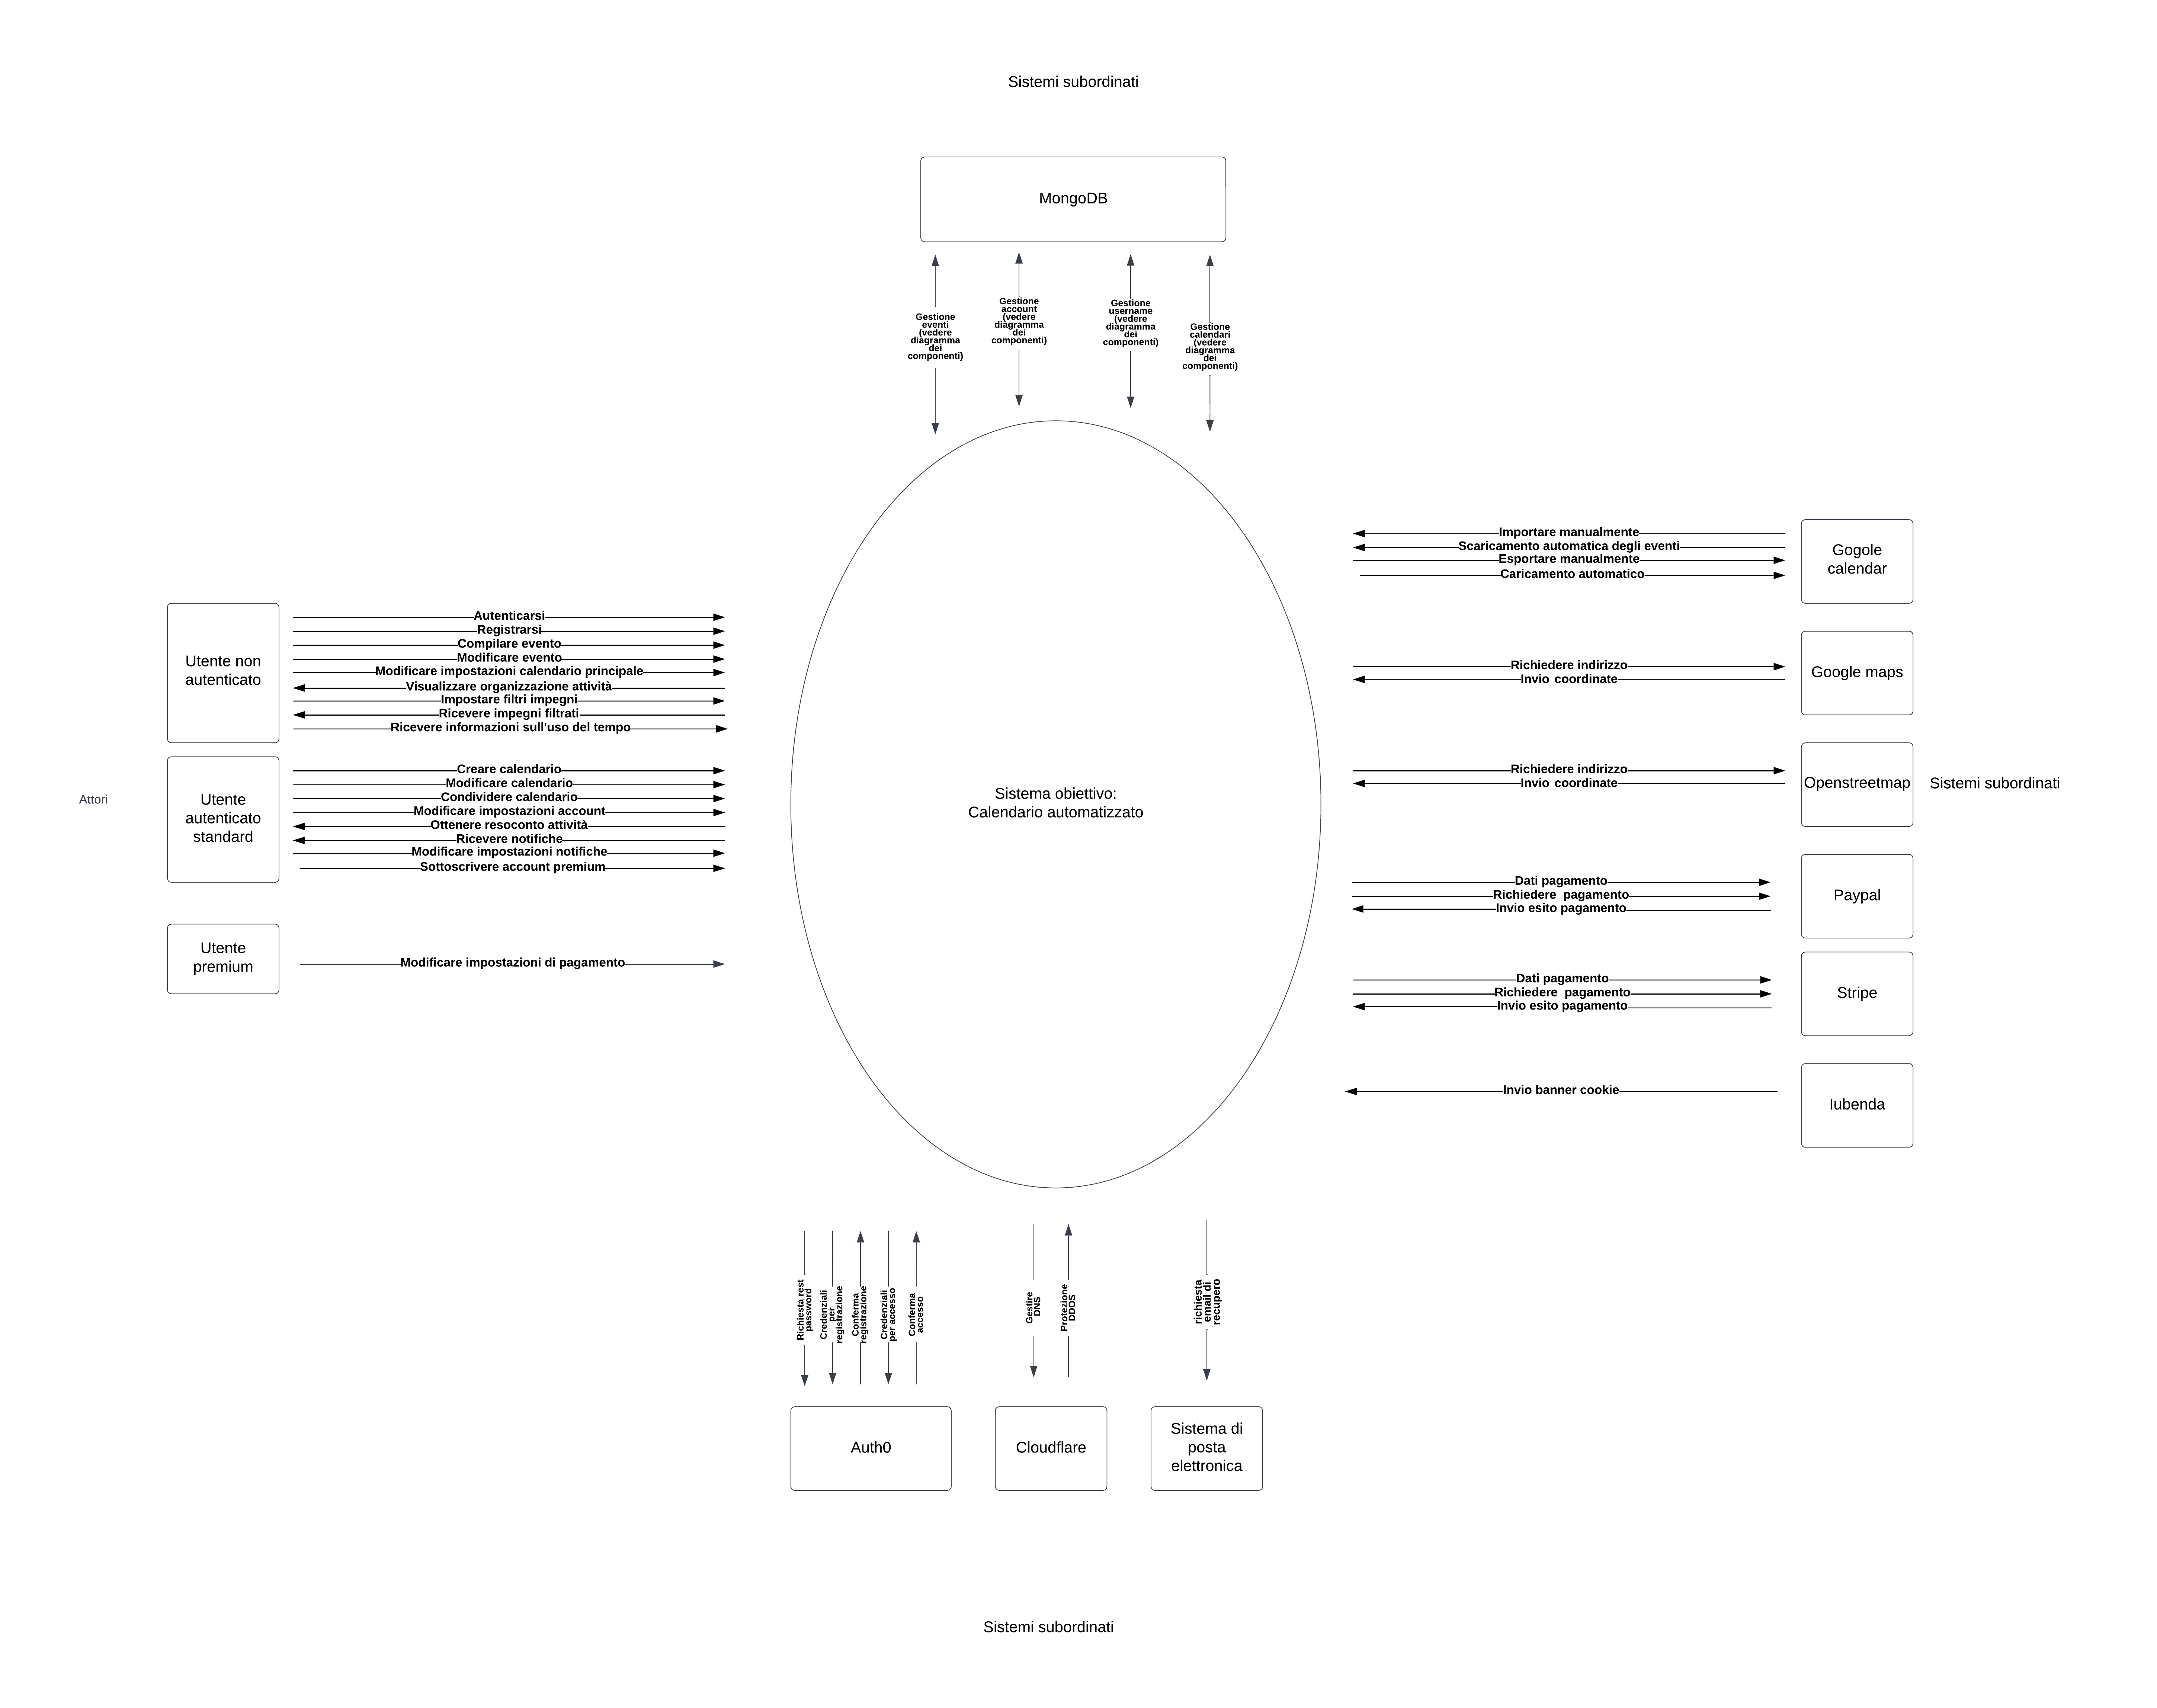
\includegraphics[width=1\textwidth]{img/Diagrammi/Contesto/DiagrammaContesto.png}
        Si prega di zoomare a piacere in modo tale di poter leggere bene le varie parti del diagramma
    \end{center}

\end{listaPersonale}